\documentclass[10pt]{IEEEtran}
\usepackage{preamble}

\begin{document}
\title{Mini-project 1: Tic Tac Toe}

\author{
   Federico Betti, Ivan Bioli\\
  \textit{CS-456 Artificial Neural Networks, EPFL Lausanne, Switzerland}
}


\maketitle


\begin{abstract}
In this report we present the results obtained from training an agent to play Tic Tac Toe both against quasi-optimal strategy (up to some user-defined degree of randomness) and by self-practice in an unsupervised fashion, then testing its performance against the optimal strategy and the fully random strategy. We use throughout the report the same notation as in the project instructions, if not stated otherwise. 
\end{abstract}
\section{Q-Learning}
\subsection*{Question 1}
\begin{figure}[H]
    \centering
    \includegraphics[scale=0.4]{code/figures/rewards_Q1.png}
    \caption{Average reward from training with $\epsilon = 0.1$ against Opt(0.5)}
    \label{plot_question1}
\end{figure}
We choose here $\epsilon = 0.1$ as this enables us to carry out a fair comparison with the decaying exploration rule later on. Smaller values of $\epsilon$ were indeed performing better. TO BE COMPLETED
\subsection*{Question 2}
In Fig. \eqref{firstplot_question2} we see that for values of $n^{*}$ such that more than half of the training episodes are played with constant $(1-\epsilon_{min})$-greedy policy, after an initial stage where action are chosen randomly more frequently and consequently the reward is lower, the majority of the actions are chosen in a greedy fashion so the average reward increases and approaches the same values seen for $n^{*} = 1$ but with the advantage of having explored more evenly the state space. 
\begin{figure}[H]
    \centering
    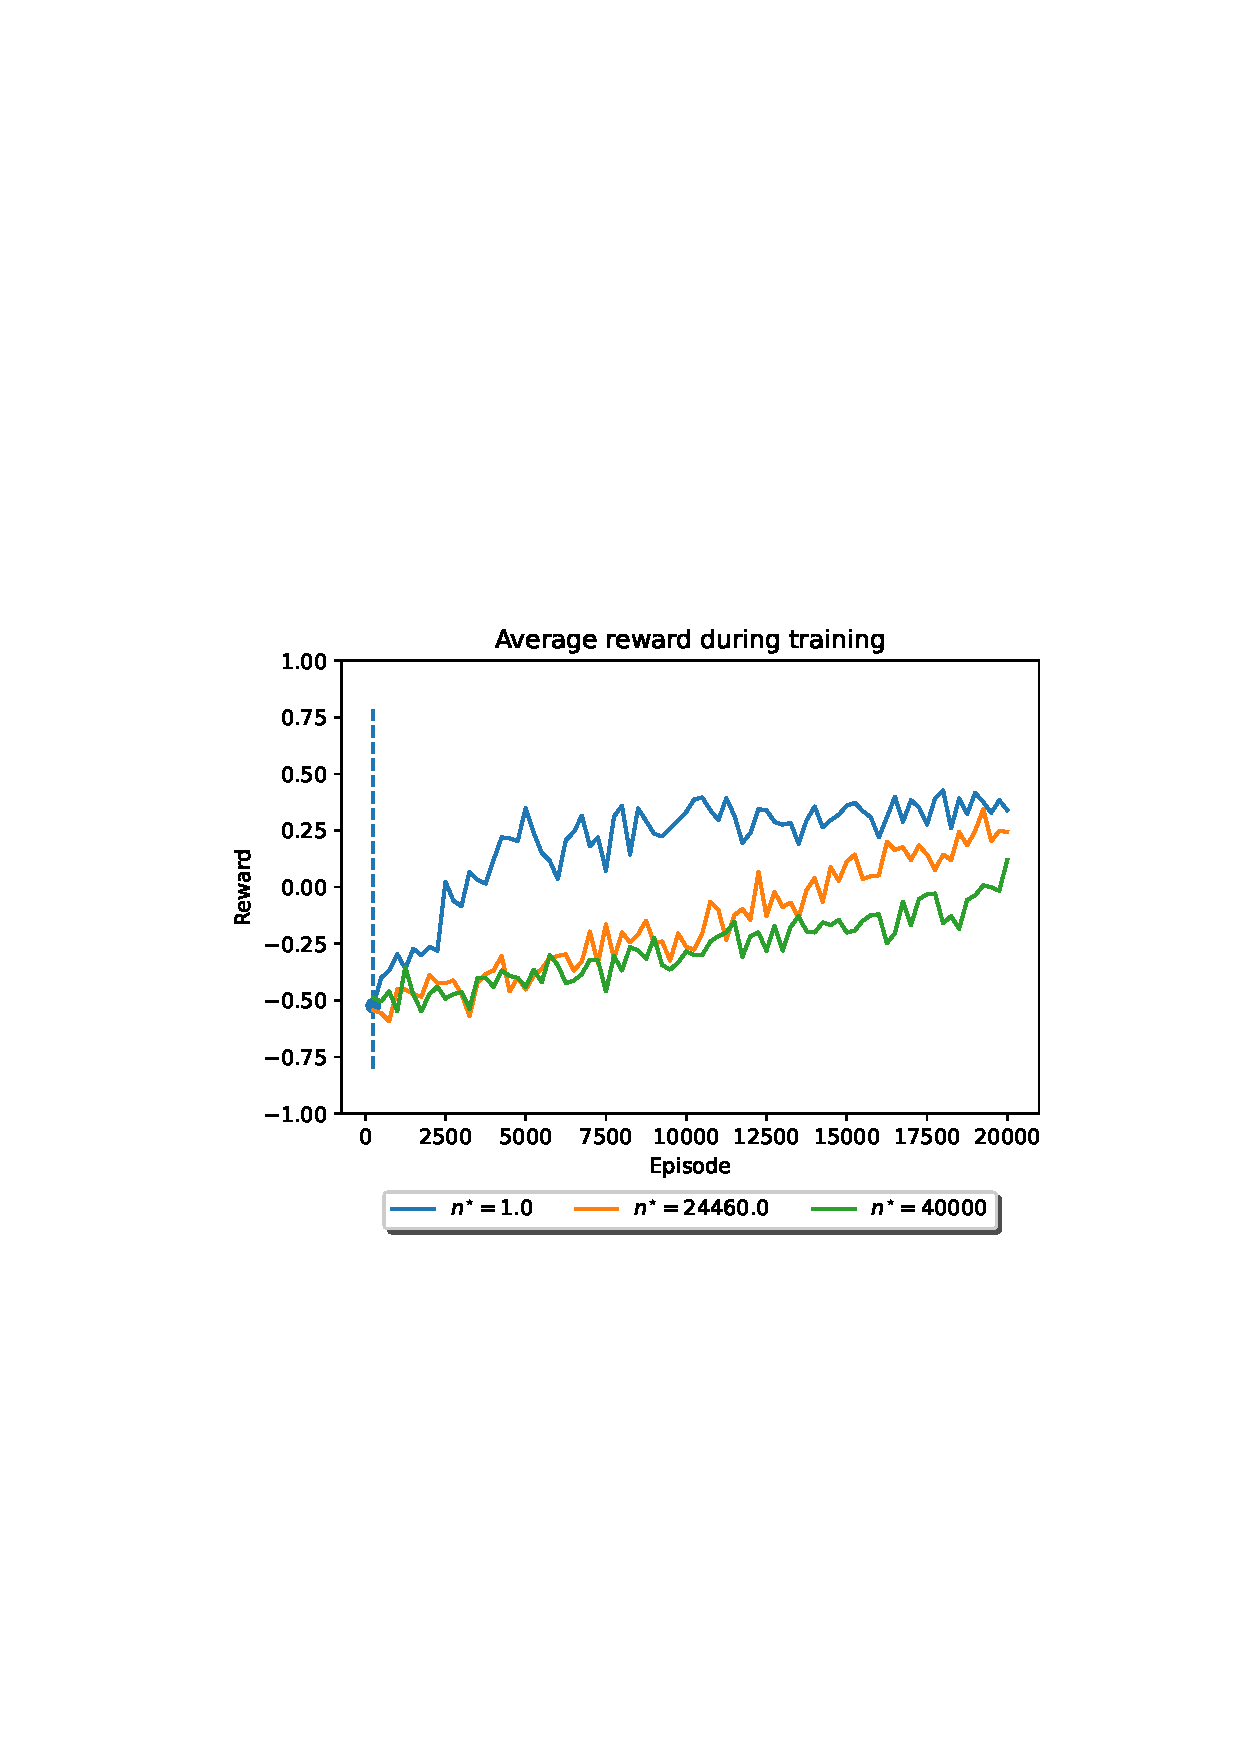
\includegraphics[scale=0.4]{code/figures/rewards_n_star_first.png}
    \caption{Average rewards from training against Opt(0.5) for higher values of $n^{*}$.}
    \label{firstplot_question2}
\end{figure}
In Fig. \eqref{secondplot_question2} we see on the other hand that for larger values of $n^{*}$ such that we never reach the constant $(1-\epsilon_{min})$-greedy policy the average reward attains lower values as the agent keeps paying the price of exploration, so it can never reach in terms of performance the $(1-\epsilon_{min})$-greedy agent. For the same reason a stronger decay of $\epsilon$ achieves eventually the same reward as observed in Fig. \eqref{plot_question1}.
\begin{figure}[H]
    \centering
    \includegraphics[scale=0.4]{code/figures/rewards_n_star_second.png}
    \caption{Average rewards from training against Opt(0.5) for smaller values of $n^{*}$: the vertical lines correspond approximately to the episode at which the agent starts eventually choosing moves with the minimum rate of exploration (for $n^{*} = 1$ this holds true from the very first episodes).}
    \label{secondplot_question2}
\end{figure}
\subsection*{Question 3}
Due to the high exploration rates, we see in Fig. \eqref{firstplot_question3} that for high values of $n^{*}$ major oscillations of $M_{opt}$: this instability is caused by the agent not really being able to play as it prioritizes exploring during the learning process. On the other hand, $M_{rand}$ increases slowly, meaning that the agent is not able to take advantage of the opponent's frequent wrong moves and coherently with the low rewards seen before. In Fig. \eqref{secondplot_question3} we observe that decreasing majorly $\epsilon$ helps stabilizing the learning process by dumping the oscillations of $M_{opt}$ and increasing faster $M_{rand}$.
\begin{figure}[H]
    \centering
    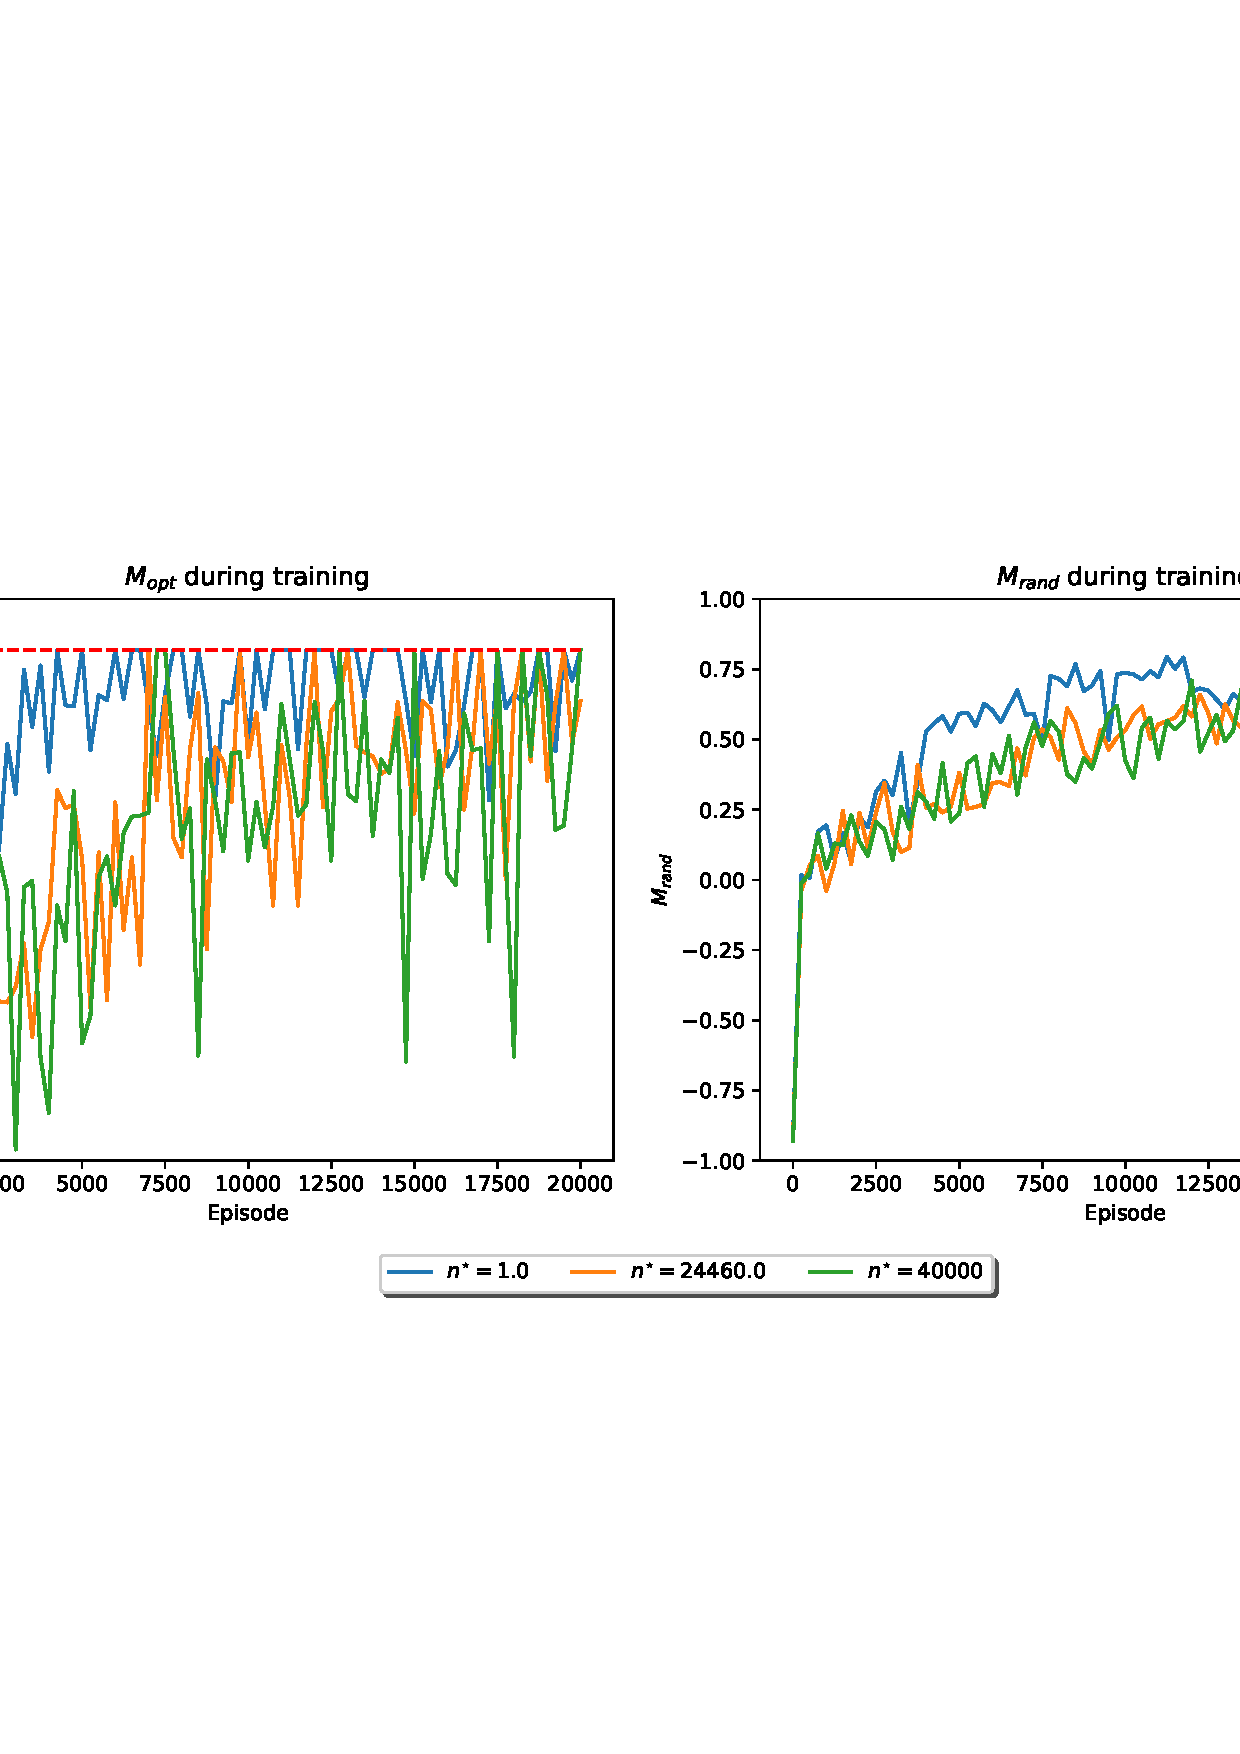
\includegraphics[width=0.49\textwidth]{code/figures/performance_n_star_first.png}
    \caption{Behaviour of $M_{opt}$ and $M_{rand}$ over the training episodes for high values of $n^{*}$}
    \label{firstplot_question3}
\end{figure}
\begin{figure}[H]
    \centering
    \includegraphics[width=0.49\textwidth]{code/figures/performance_n_star_second.png}
    \caption{Behaviour of $M_{opt}$ and $M_{rand}$ over the training episodes for small values of $n^{*}$}
    \label{secondplot_question3}
\end{figure}
\subsection*{Question 4}
\subsection*{Question 5}
\subsection*{Question 6}
\subsection*{Question 7}
\subsection*{Question 8}
\subsection*{Question 9}
\subsection*{Question 10}
\section{Deep Q-Learning}
\subsection*{Question 11}
\subsection*{Question 12}
\subsection*{Question 13}
\subsection*{Question 14}
\subsection*{Question 15}
\subsection*{Question 16}
\subsection*{Question 17}
\subsection*{Question 18}
\subsection*{Question 19}
\subsection*{Question 20}
\subsection*{Question 21}
\nocite{*}
\end{document}